\subsection{简单几何体的三视图}\label{subsec:czjh2-8-4}

在生产中所遇到的零件,形状虽然各不相同,但它们一般是由一些简单几何体(柱体、锥体、台体和球体等)组合或切割而成的。
因此熟悉简单几何体的视图是非常必要的,同时这些视图又是工程、机械等制图、识图的基础。
前面已学了一部分简单几何体的视图,这里再介绍棱柱、棱锥、棱台的三视图。


\subsubsection{棱柱的三视图}

画简单体的三视图,一般先画底。以正六棱柱的三视图为例,如果正六棱柱如图 \ref{fig:czjh2-8-16} (a) 这样放置,
那么应该先画俯视图,然后再画其他的视图。

具体画法同前面的三视图画法类似,同学们可按图 \ref{fig:czjh2-8-16} (b)、(c)、(d) 一步步自行分析。
描好轮廓线后,擦去不必要的辅助线,再标注尺寸(图 \ref{fig:czjh2-8-16} (e)),这样,一张图才算完成。

\begin{figure}[htbp]
    \centering
    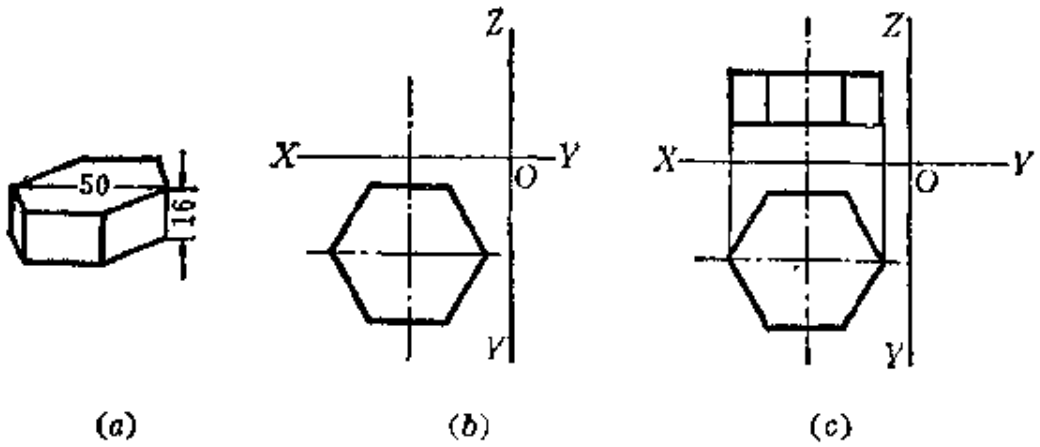
\includegraphics[width=12cm]{../pic/czjh2-ch8-16-1.png}
    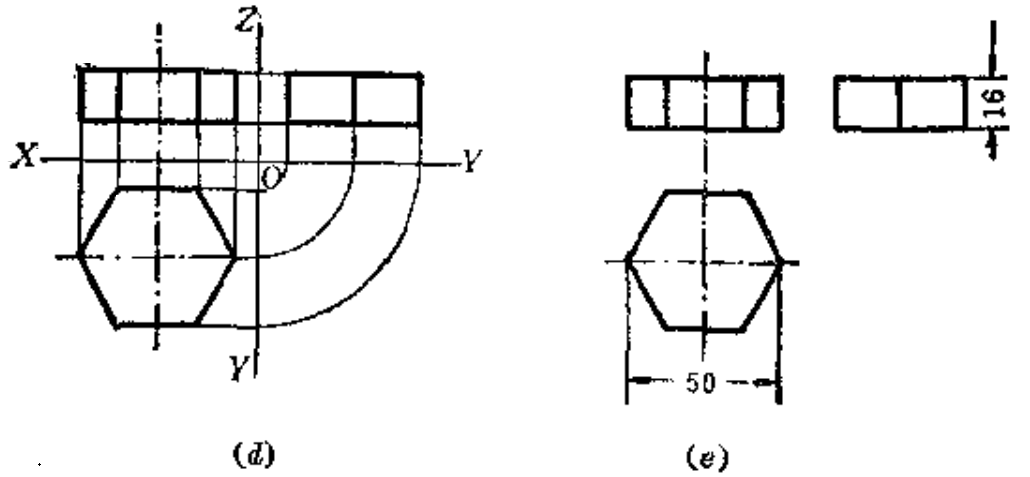
\includegraphics[width=12cm]{../pic/czjh2-ch8-16-2.png}
    \caption{}\label{fig:czjh2-8-16}
\end{figure}

如果正六棱柱如图 \ref{fig:czjh2-8-17} 这样放置,这时画三视图应先画主视图,然后再画其他视图,具体画法与上面一样。

\begin{figure}[htbp]
    \centering
    \begin{minipage}[b]{4cm}
        \centering
        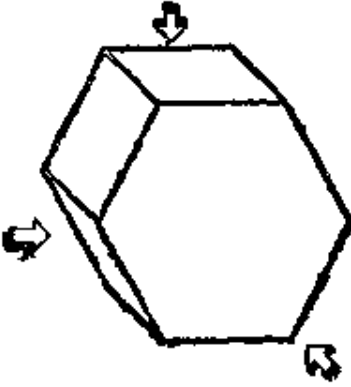
\includegraphics[width=3.5cm]{../pic/czjh2-ch8-17.png}
        \caption{}\label{fig:czjh2-8-17}
    \end{minipage}
    \qquad
    \begin{minipage}[b]{10cm}
        \centering
        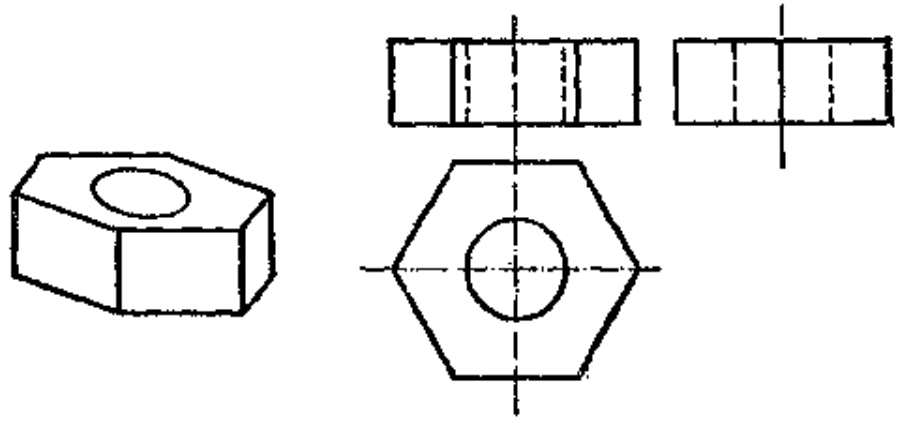
\includegraphics[width=9cm]{../pic/czjh2-ch8-18.png}
        \caption{}\label{fig:czjh2-8-18}
    \end{minipage}
\end{figure}

六角螺母毛坯的三视图,可以看作正六棱柱和圆柱的两个三视图的组合,如图 \ref{fig:czjh2-8-18}。
因为孔的轮廓线是看不见的,所以在主视图与左视图上都要画虚线。


\subsubsection{棱锥、棱台的三视图}

棱锥与棱台的视图画法与棱柱的视图画法是一样的,也是先画底的视图,然后很据三视图规律画出其他的视图。
这里的画法请同学们自行分析。为了便于同学们考虑,图中的辅助线都保留着。

底面边长为 30 mm、高为 30 mm 的正三棱锥的三视图,如图 \ref{fig:czjh2-8-19} 所示。

\begin{figure}[H]%[htbp]
    \centering
    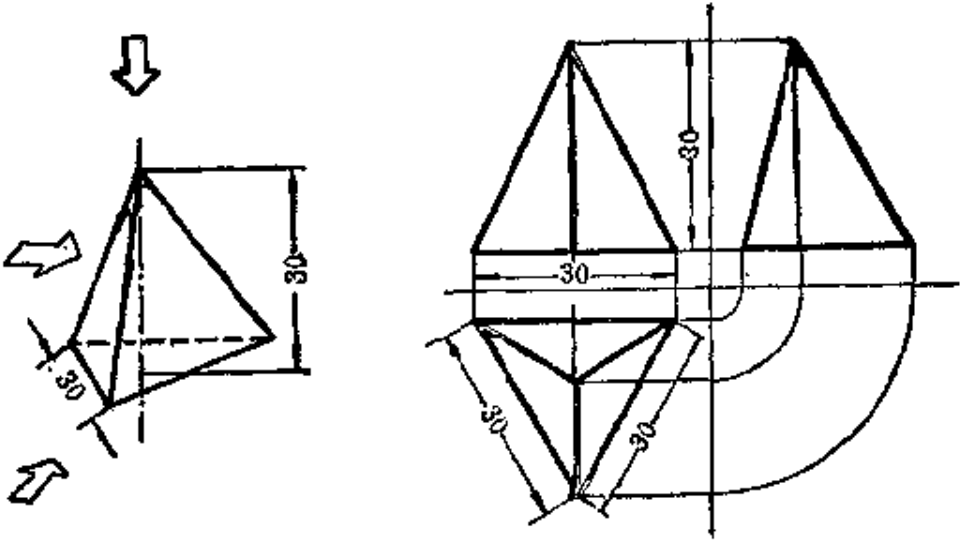
\includegraphics[width=12cm]{../pic/czjh2-ch8-19.png}
    \caption{}\label{fig:czjh2-8-19}
\end{figure}

上底面边长为 20 mm,下底面边长为 40 mm,高为 30 mm 的正四棱台的三视图,如图 \ref{fig:czjh2-8-20} 所示。

\begin{figure}[htbp]
    \centering
    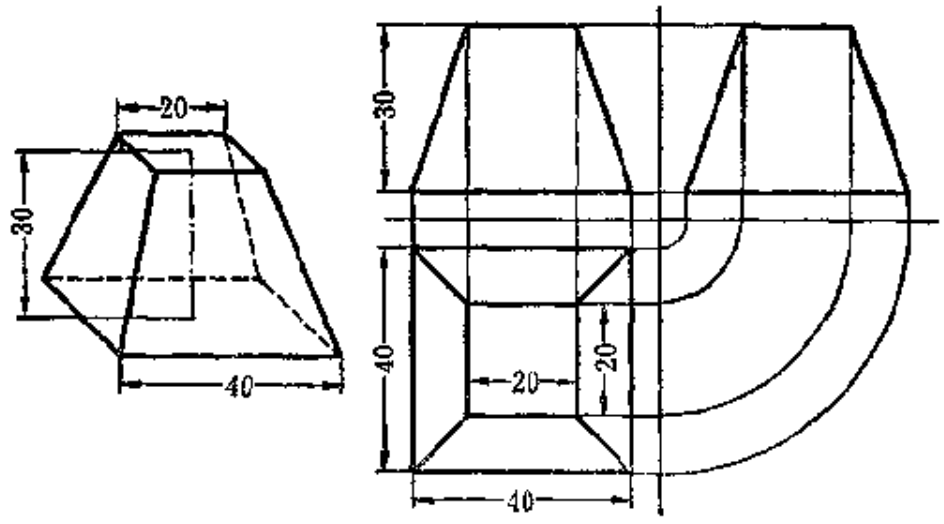
\includegraphics[width=12cm]{../pic/czjh2-ch8-20.png}
    \caption{}\label{fig:czjh2-8-20}
\end{figure}

视图要求简明扼要,通常要使主视图能比较全面地反映物体的特征,而且在不影响表达清楚的前提下,
可以省略左视图或俯视图。如球、圆柱等旋转体在图纸中常用一个视图来表示(如图 \ref{fig:czjh2-8-21} (a)、(b));
棱柱、棱锥、棱台等几何体,常用二视图来表示。
当然也有些复杂的零件用三视图还不能够清楚地表示出来,需要用其他的视图加以补充,这里不再详细说明了。

\begin{figure}[htbp]
    \centering
    \begin{minipage}[b]{10cm}
        \centering
        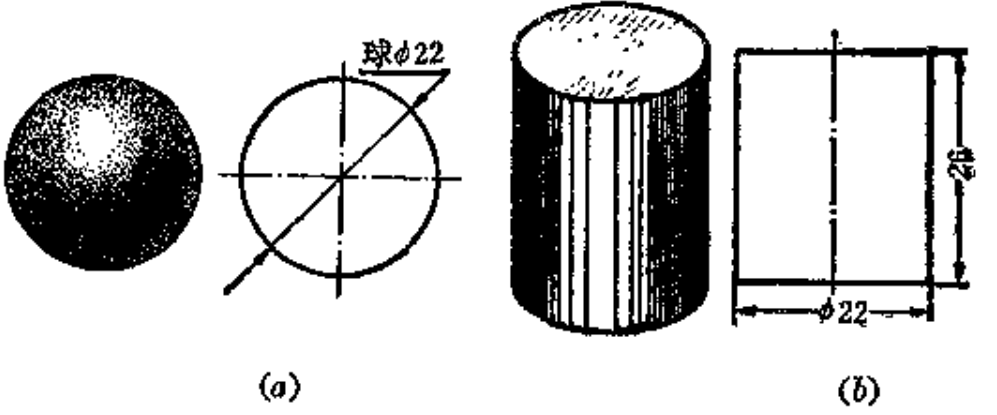
\includegraphics[width=10cm]{../pic/czjh2-ch8-21.png}
        \caption{}\label{fig:czjh2-8-21}
    \end{minipage}
    \qquad
    \begin{minipage}[b]{4cm}
        \centering
        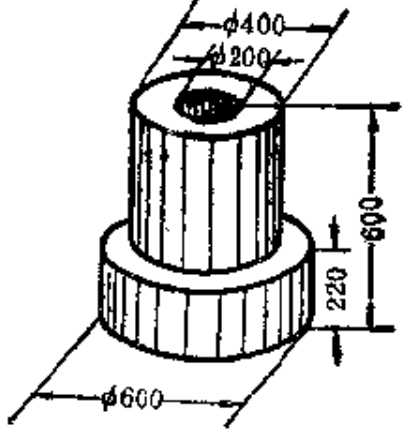
\includegraphics[width=4cm]{../pic/czjh2-ch8-subsec4-lx-01.png}
        \caption*{(第 1 题)}
    \end{minipage}
\end{figure}

\begin{lianxi}

\xiaoti{如果一个零件的尺寸非常大(或者非常小),那么画视图时怎么办?
    试画出一个铸件的三视图,尺寸如图(铸件上面是一个圆柱,下面也是一个圆柱,
    中间挖去一个直径为 200 mm 的圆柱,直通到底)。
    (提示:用适当的比例尺画图,尺寸仍注原件实际尺寸。)
}

\xiaoti{添线补全下列三视图。}

\begin{figure}[htbp]
    \centering
    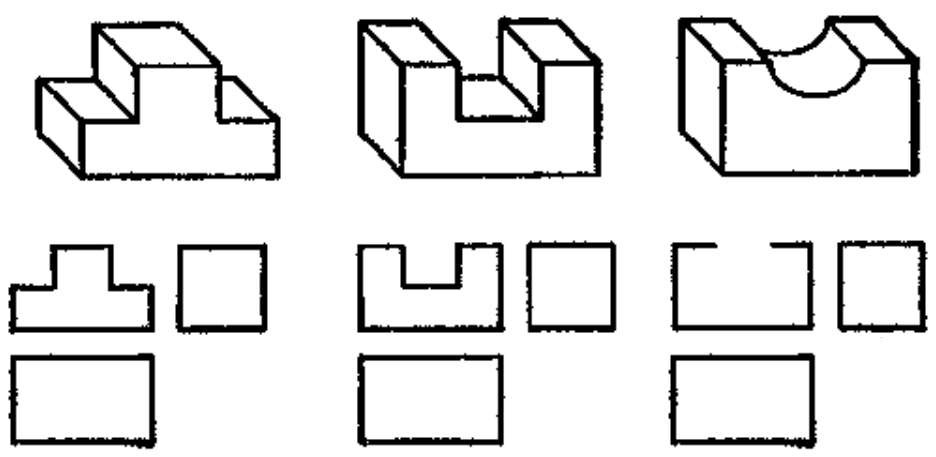
\includegraphics[width=11cm]{../pic/czjh2-ch8-subsec4-lx-02.png}
    \caption*{(第 2 题)}
\end{figure}

\xiaoti{找出下列直观图对应的三视图,在括号中填上对应的数码。}

\begin{figure}[htbp]
    \centering
    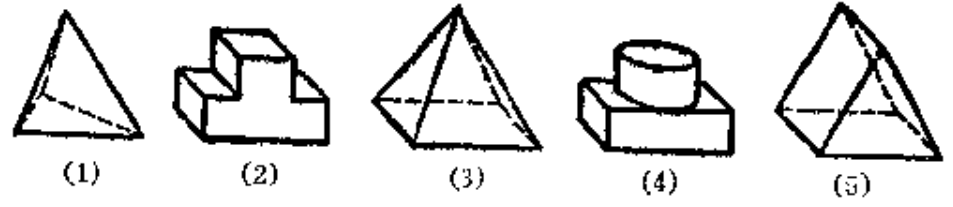
\includegraphics[width=11cm]{../pic/czjh2-ch8-subsec4-lx-03-1.png}
    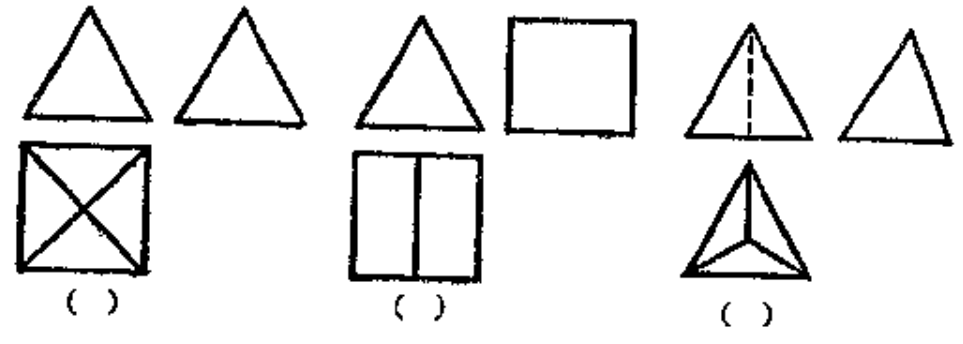
\includegraphics[width=11cm]{../pic/czjh2-ch8-subsec4-lx-03-2.png}
    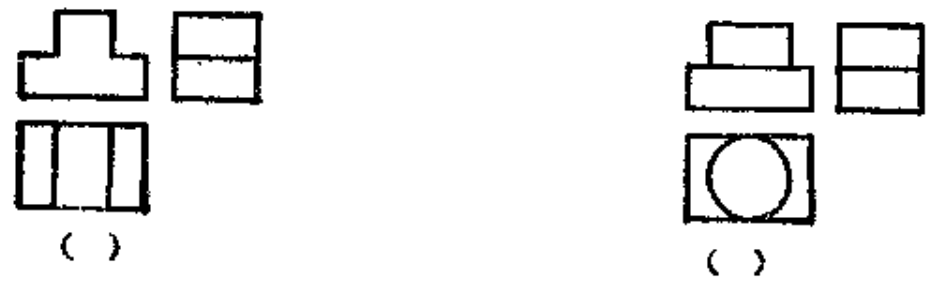
\includegraphics[width=11cm]{../pic/czjh2-ch8-subsec4-lx-03-3.png}
    \caption*{(第 3 题)}
\end{figure}

\end{lianxi}

